\documentclass[11pt, oneside]{article}   	% use "amsart" instead of "article" for AMSLaTeX format
\usepackage{geometry}                		% See geometry.pdf to learn the layout options. There are lots.
\geometry{letterpaper}                   		% ... or a4paper or a5paper or ... 
%\geometry{landscape}                		% Activate for rotated page geometry
%\usepackage[parfill]{parskip}    		% Activate to begin paragraphs with an empty line rather than an indent

\usepackage{graphicx}				% Use pdf, png, jpg, or eps§ with pdflatex; use eps in DVI mode

%maths							% TeX will automatically convert eps --> pdf in pdflatex		
\usepackage{amssymb}
\usepackage{amsmath}
\usepackage{mathtools}
\usepackage[most]{tcolorbox}

%pgfplots
\usepackage{pgfplots}

%images
\graphicspath{{/Users/devaldeliwala/undergrad/23s/textbook/img}}

%tikz
\usepackage{tikz}
\usepackage{bbold} 					% for \mathbb
\usepackage[outline]{contour} 			% glow around text
\usetikzlibrary{arrows.meta} 			% to control arrow size
\usepackage{xcolor} 					% for colored text
\tikzset{>=latex} 					% for LaTeX arrow head
\contourlength{1.2pt}

\newcommand\LP{{\color{mydarkblue}P}} %\Lambda_\mathrm{P}
\newcommand\LT{{\color{mydarkred}T}} 	%\Lambda_\mathrm{T}
\colorlet{myred}{red!60!black}
\colorlet{myblue}{blue!60!black}
\colorlet{mygreen}{green!60!black}
\colorlet{mydarkblue}{blue!40!black}
\colorlet{mydarkred}{red!40!black}
\colorlet{mydarkgreen}{green!40!black}
\colorlet{mydarkpurple}{blue!50!red!50!black}
\tikzstyle{myarr}=[-{Latex[length=4,width=3]}]

%table of contents
\setcounter{tocdepth}{4}
\setcounter{secnumdepth}{4}


\title{Physics 89}
\author{deval deliwala}
%\date{}							% Activate to display a given date or no date

\begin{document}
\maketitle
%\section{}
%\subsection{}

\begin{center}
\scriptsize{Adapted from Mathematics for Physicists: Introductory Concepts and Methods by Atland \& Delft}
\end{center}

\begin{center}
\vspace{50px}
\hspace{50px}
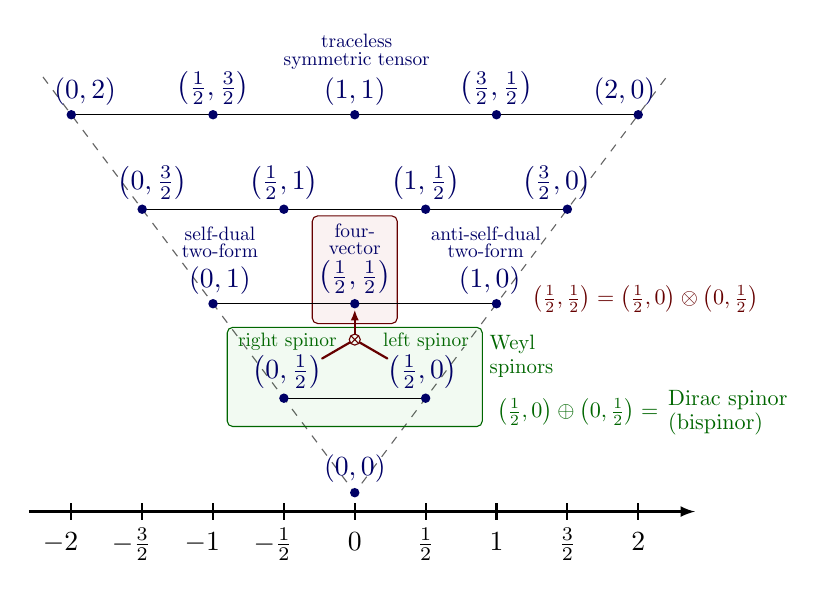
\begin{tikzpicture}[x=1.8cm,y=1.2cm]
  \def\N{4}      % number of spin states
  \def\r{0.07cm} % radius otimes
  \def\repr#1{   % format simple fraction
    \pgfmathsetmacro{\double}{int(2*#1)}
    \pgfmathsetmacro{\sign}{ifthenelse(#1<0,"-","")}
    \pgfmathparse{int(mod(\double,2))}
    \ifnum0=\pgfmathresult\relax % even
      \pgfmathprintnumber{#1}
    \else % odd
      \sign % sign
      \pgfmathparse{abs(int(\double))}
      \frac{\pgfmathprintnumber{\pgfmathresult}}{2}
    \fi
    \phantom{\sign} % for centered alignment
  }
  
  % AXIS
  \begin{scope}[shift={(0,-0.2)}]
    \draw[->,thick] (-\N/2-0.3,0) -- (\N/2+0.4,0); %node[right=-1] {$S$};
    \foreach \j [evaluate={\x=\j/2; \m=\j/2;}] in {-\N,...,\N}{ % ticks
      \draw[thick] (\x,0.09) --++ (0,-0.18)
        node[below=-1] {\strut$\repr{\m}$}; 
    }
  \end{scope}
  
  % LABELS Dirac spinor
  \draw[dashed,opacity=0.6] (-1.1*\N/2,1.1*\N) -- (0,0) -- (1.1*\N/2,1.1*\N);
  \draw[mydarkgreen,fill=mygreen,fill opacity=0.05,rounded corners=2]
    (-0.9,0.7) rectangle (0.9,1.75)
    node[mydarkgreen,below right,align=left,opacity=1,scale=0.75] {Weyl\\spinors};
  \node[mydarkgreen,scale=0.8,below right] at (0.95,1.2)
    {$\left(\frac{1}{2},0\right)\oplus\left(0,\frac{1}{2}\right)
       = \!\! \begin{array}{l}
           \text{Dirac spinor}\\[-0.5mm]
           \text{(bispinor)}
         \end{array}$};
  %\node[mydarkgreen,scale=0.8,below,align=center] at (1.55,0.68)
  %  {Dirac spinor\\[-3](bispinor)};
  %\node[mydarkgreen,scale=0.8,below,align=center] at (2.58,0.68)
  %  {four-\\[-3]vector};
  %\node[mydarkgreen,scale=0.8,below right] at (1.5,2.2)
  %  {$(1,0)\oplus(0,1) = \text{adjoint}$}; % parity-invariant 2-form field
  
  % LABELS four-vector
  \draw[mydarkred,fill=myred,fill opacity=0.05,rounded corners=2]
    (-0.3,1.79) rectangle (0.3,2.93);
  \node[mydarkred,scale=0.8,right] at (1.2,2.05)
    {$\left(\frac{1}{2},\frac{1}{2}\right) = %\cong
      \left(\frac{1}{2},0\right)\otimes\left(0,\frac{1}{2}\right)$};
  
  % DOTS
  \foreach \j [evaluate={\y=\j;}] in {0,...,\N}{
    \draw (-\j/2,\y) --++ (\j,0);
    \foreach \i [evaluate={
      \m=\i-\j/2;
      \L=\i/2; % left representation
      \R=\j/2-\i/2; % right representation
      \x=\m; % x position
      \myshift=((\i==0||\i==\j)?-2.5*\x:0);
    }] in {0,...,\j}{
      \fill[mydarkblue] (\x,\y) circle (0.06cm);
      \node[mydarkblue,right=\myshift,above]
        %,fill=white,text opacity=1,fill opacity=0.5,inner sep=0.5,outer sep=3
        (P\j-\i) at (\x,\y) {$\left(\repr{\L},\repr{\R}\right)$};
    }
  }
  
  % ARROWS & OTIMES
  \draw[thick,mydarkred,line cap=round]
    (-0.23,1.42) -- (0,1.62) coordinate (A) -- (0.23,1.42);
  \draw[myarr,thick,mydarkred,line cap=round]
    (A) -- (0,1.94);
  \draw[mydarkred,line width=0.4,fill=mygreen!5] % circle
    (A) circle(\r);
  \draw[mydarkred,line width=0.4] % cross
    (A)++(45:\r) --++ (-135:2*\r)
    (A)++(135:\r) --++ (-45:2*\r);
  
  % LABELS
  \node[mydarkgreen,scale=0.7,above=6]
    at (P1-0) {\strut\contour{mygreen!5}{right spinor}};
  \node[mydarkgreen,scale=0.7,right=2,above=6]
    at (P1-1) {\strut\contour{mygreen!5}{left spinor}};
  \node[mydarkblue,scale=0.7,above=8,align=center]
    at (P2-0) {self-dual\\[-3]two-form};
  \node[mydarkblue,scale=0.7,above=8,align=center]
    at (P2-1) {four-\\[-3]vector};
  \node[mydarkblue,scale=0.7,left=2,above=8,align=center]
    at (P2-2) {anti-self-dual\\[-3]two-form};
  \node[mydarkblue,scale=0.7,right=1,above=8,align=center]
    at (P4-2) {traceless\\[-3]symmetric tensor};
  
\end{tikzpicture}
\end{center}

\newpage

\tableofcontents

\newpage

\section{Chapter 1: Linear Algebra} 
\subsection{L1: Mathematics before Numbers} 
\subsubsection{L1.1: Sets and Maps} 
\paragraph{Sets} \mbox{} \\ \\
 A set is a container holding certain elements. Formally, one writes $a \in A$ to indicate that \textbf{a} is an element of set \textit{A} and $A = \{a, b, c, ... \}$. Building upon this definition of a set and its elements, \\

$\rightarrow$ We write $A = \{\}$ or $A = \emptyset$ to denote the \textbf{emptyset} \\

$\rightarrow$ A \textbf{subset} of $A$, denoted by $B\subset A$, contains some of the elements of $A$, for example, $B = \{a, b\} \subset A$. We may write $B \subseteq A$ if we want to indicate that the subset $B$ may actually be equal to $A$, or $B \subsetneq A$ if this is not the case \\

$\rightarrow$ The \textbf{union} of two sets is denoted by $\cup$, for example, $\{a, b, c\} \cup \{c, d\} = \{a, b, c, d\}$. The \textbf{intersection} is denoted by $\cap$, for example $\{a, b, c\} \cap \{c, d\} = \{c\}$ \\

$\rightarrow$ The removal of a subset $B \subset A$ from a set $A$ that results in the \textbf{difference set} denoted by $A/B$. For example, $\{a, b, c, d\} / \{c\} = \{a, b, d\}$ \\ 

$\rightarrow$ We will often define sets by \textbf{conditional rules} where $\text{set} = \{ \text{elements} | \text{rule} \}$. For example, with $A = \{1,2,3,4,5,6,7,8,9,10\}$ the set of all even integers up to 10 could be defined as $B = \{a \in A | a/2 \in A\} = \{2,4,6,8,10\}$. \\

$\rightarrow$ Given two sets $A$ and $B$, we define their \textbf{Cartesian Product} as 
\[ A \times B = \{(a,b) | a \in A, b \in B\}, \]
i.e. the container of all pairs formed by elements of $A$ and $B$. 

$\rightarrow$ The number of elements in a set is called its \textbf{cardinality}, which can be finite or infinite. Among those that are infinite we can distinguish between 'countable' and 'uncountable' sets. A set is \textbf{countable} if you can come up with a way to number its elements, for example, the set of even integers. \\

$\rightarrow$ Sometimes it is useful to organize sets in terms of \textbf{equivalence classes} expressing the equality $a \sim b$ of two elements relative to a certain criterion, $R$. For example let $A$ be the set of all your relatives and let the criterion, $R$, be their sex. If $a$ and $b$ are both female or both male, we write $a \sim b$ An equivalence relation has the following properties: \\\\
\begin{tcolorbox}[colback = red!5!white, colframe = red!50!black, title
  = Equivalence Classes]

$\rightarrow$ \textbf{reflexivity}: $a \sim a$, every element is equivalent to itself. \\
$\rightarrow$ \textbf{symmetry}: $a \sim b$ implies $b \sim a$ \\ 
$\rightarrow$ \textbf{transitivity}: $a \sim b$ and $b \sim c$ implies $a \sim c$. 

\end{tcolorbox}

The subset of all elements equivalent to a given reference element $a$ is
called an \textbf{equivalence class} and denoted $[a] \subset A$. In the
example of relatives and their sex, there are two equivalencei classes, for example $A = [\text{dad}] | [\text{mom}]$, one also might relabel $[\text{mom}] = [\text{aunt}]$. The set of all equivalence classes relative to a relation $R$ is called its \textbf{quotient set} and is denoted by $A/R$. The quotient set $A/R = \{[\text{dad}], [\text{mom}]\}$ would have two elements, the class of males and females. \\

\vspace{20px}

\textbf{Example} Consider the set of integers, and pick some integer $q$. Let any two integers be equivalent if they have the same remainder under division by $q$. \\

The equivalence class of all integers with the same remainder $r$ under division by $q$ is 

\[ [r] = \{ p \in \mathbb{Z} | p \text{ mod } q = r\} \]

There are $q$ such equivalence classes, and the set of these classes is denoted by 

\[ \mathbb{Z}_q \equiv \mathbb{Z} / q\mathbb{Z} = \{[0], [1], ..., [q-1]\} \]

\paragraph{Maps} \mbox{} \\ \\ 

Suppose you have two sets, $A$ and $B$, together with a rule, $F$, such that each element of $A$ has a corresponding element in $B$, where $F(a) \equiv b \in B$. Such a rule is called a \textbf{map}, which are specified by the following notation: 

\[ F: A \rightarrow B \]
\[ a \mapsto F(a) \] 

The set $A$ is called the \textbf{domain} of the map and $B$ is its \textbf{codomain}. An element $a \in A$ fed into the map is called an \textbf{argument} and $F(a)$ is its \textbf{image}. 

\[ \text{domain} \rightarrow \text{codomain} \]
\[ \text{argument} \mapsto \text{image} \]

The \textbf{image} of $A$ under $F$, denoted by $F(A)$, is the set containing
all image elements of $F: F(A) = \{ F(a) | a \in A\} \subseteq B$. \\

\begin{tcolorbox}[colback = blue!5!white, colframe = blue!50!black, title
  = Different Tives] 
  
$\rightarrow$ A map is called \textbf{surjective} if its image covers all of $B, F(A) = B$, where any element of the codomain is the image of \textit{at least} one element of the domain.  \\
\indent $\rightarrow$ A map is called \textbf{injective} if every element of the codomain is the image of \textit{at most} one element of the domain. \\
\indent $\rightarrow$ A map is called \textbf{bijective} if its both surjective
and injective, if every element of the codomain is the image of exactly one
element of the domain. This is called a \textit{one-to-one} relationship. This allows the map to also establish an \textbf{inverse map}, $F^{-1}: B \rightarrow A$ such that $F^{-1}(F(a)) = a$ for every $a \in A$ \\ 

\end{tcolorbox}

\begin{center}
  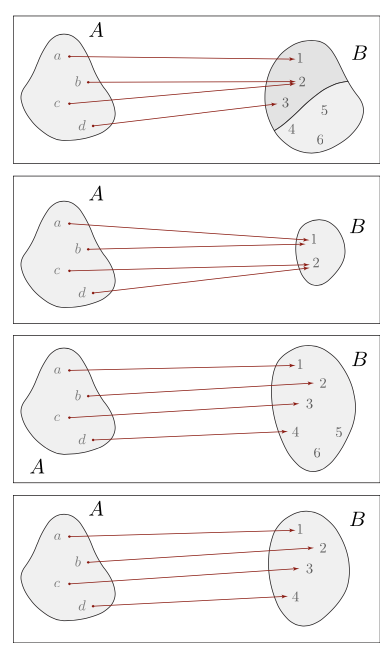
\includegraphics[width = 5cm]{ss.png}
\end{center}

Given two maps, $F: A \rightarrow B$ and $G: B \rightarrow C$, their \textbf{composition} is defined by using the image element of one as an argument for the other: 

\[ G \circ F: A \rightarrow C\] 
\[a \mapsto G(F(a)) \] \\

\subsubsection{L1.2: Groups} 

The minimal structure which brings a set to life in terms of different operations between its elements is called a \textbf{group}. Let $A$ be a set and consider an \textbf{operation} denoted by '$\cdot$', that assigns every pair of elements $a$ and $b$ in $A$ another element, denoted by $a \cdot b$: 

\[ \cdot : A \times A \rightarrow A \]
\[(a,b) \mapsto a\cdot b\] 

The set $A$ and composition rule '$\cdot$' form a group, denoted by $G=(A, \cdot)$, provided that the following four \textbf{group axioms} are satisfied: \\

\begin{tcolorbox}[colback=red!5!white, colframe=red!50!black, title = Group Axioms]
$\rightarrow$ Closure: $a\cdot b$ is also in $A$ \\
$\rightarrow$ Associativity: $(a \cdot b) \cdot c = a \cdot (b \cdot c)$ \\
$\rightarrow$ Neutral Element: there exists an element $e$ in $A$ such that $e \cdot a = a \cdot e = a$\\
$\rightarrow$ Inverse Element: for each $a$ in $A$ there exists $b$ in $A$ such that $a \cdot b = b \cdot a = e$ \\
\end{tcolorbox}

\subsubsection{L1.3: Fields}

A set for which both addition and multiplication is defined as separate operations is called a \textbf{field}. Formally, a field is a triple $F \equiv (A, +, \cdot)$, comprising a set $A$ and two composition rules, addition and multiplication. The addition of the inverse element is known as \textbf{subtraction}. The multiplication by inverse is known as \textbf{division}. 

\textbf{Example} \\
The integers ,$\mathbb{Z}$, do not form a field because multiplication always yields an integer, but division generally does not. 

\paragraph{Complex Numbers} 

Addition and multiplication is defined by: 

\[ z + z' = (x + iy) + (x' + iy') \equiv (x+ x') + i(y + y') \] 
\[ zz' = (x+ iy)(x'+iy') \equiv (xx' - yy') + i(xy' + yx') \]

The \textbf{complex conjugate} is defined by

\[ \bar{z} \equiv x = iy \] 

Therefore, 

\[ z\bar{z} = x^2 + y^2 \]

\subsection{L2: Vector Spaces}

\subsubsection{L2.2: The standard vector space $\mathbb{R}^n$} \mbox{} \\
\[
\mathbb{R}^n \equiv
\left \{ \vec{x} = 
\begin{pmatrix}
x^1 \\ x^2 \\ \vdots \\ x^n
 \end{pmatrix} 
 \Bigg| x^1, x^2, \cdots, x^n \in \mathbb{R} \right\}.
 \] \\
 
 \textbf{Addition} of vectors is defined by \\
 
 \[ \begin{pmatrix} 
 1.5 \\ 2 \\ 0 \end{pmatrix} = \begin{pmatrix} 0.5 \\ -3 \\1 \end{pmatrix} + \begin{pmatrix}  1\\5\\-1 \end{pmatrix} \]\\
 
  \textbf{Multiplication} of a vector, by a scalar is defined by  \\
  
  \[ 2 \begin{pmatrix} 1.5\\2\\0 \end{pmatrix} = \begin{pmatrix} 3\\4\\0\end{pmatrix}. \] \\
  
  Notice that the vectors can not be multiplied with each other. 

\subsubsection{L2.2 General Definition of Vector Spaces}

In the theory of quantum mechanics, \textit{functions} are considered as
vectors. Vectors do not always need to be lines with arrows. \\

Although a function does not resemble an arrow, it meets criteria defining
a vector and this analogy plays an important role in numerous applications. \\

However, let us first introduce the general vector space definition. 

\paragraph{Vector Space Definition} 

The defining property of vectors is that they can be added to each other and
multiplied by elements of a number field $\mathbb{F}$. The formal definition of
a set of such objects is \\

An $\mathbb{F}$-\textbf{vector space} is a triple, $(V, +, \cdot)$, consisting
of a set, $V$, a \textbf{vector addition} rule, 

\begin{align*}
  + : &V \times V \mapsto V \\
      &(\vec{v}, \vec{w} ) \mapsto \vec{v} + \vec{w}. 
\end{align*}\\ 

and a rule for \textbf{multiplication by scalars}

\begin{align*}
  \cdot :& \mathbb{F} \times V \mapsto V \\
  &(a, \vec{v}) \mapsto \vec{v} + \vec{w}. 
\end{align*}\\ 

such that the following \textbf{vector space axioms} hold: (i) the addition of
vectors, $(V,+)$, the neutral element of addition, $\vec{0}$, is called a null
vector; the inverse element of a vector is called the negative vector,
$-\vec{v}$. (ii) Scalar Multiplication satisfies the following rules, $\forall
a, b \in \mathbb{F}, \textbf{v}, \textbf{w} \in V$: \\

\begin{tcolorbox}[colback = blue!5!white, colframe = blue!50!black, title
  = Multiplication Rules]
  \begin{align*}  
&1. \hspace{10px}(a+b)\vec{v} = a\vec{v}  + b\vec{v} \\
&2. \hspace{10px}a(\vec{v} + \vec{w}) = a\vec{v} + a\vec{w} \\
&3. \hspace{10px}(ab)\vec{v} = a(b\vec{v}) \\ 
&4. \hspace{10px}1\vec{v} = \vec{v}
  \end{align*}
\end{tcolorbox}


\paragraph{Covariant Notation}

Below we will frequently consider sums  $\vec{v_1}x^1 + \vec{v_2}x^2 + \dots
$ of vectors $\vec{v_1},\vec{v_2},\dots$ with coefficients $x^1,x^2,\dots$.
Superscript and subscript indices are called  \textbf{contravariant indices}
and \textbf{covarient indices}, respectively. Notation adopting this index
positioning convention is called \textbf{covariant notation}  

\end{document}  
